\documentclass[../main.tex]{subfiles}

\begin{document}

\onehalfspacing

Es importante mencionar que, los datos del estudio son del año 2012 por lo que no es posible generalizar a dinámicas actuales. La tecnología y necesidades hoy en día han cambiado considerablemente, así como la sociedad ha modificado las políticas permitiendo una alteración al comportamiento [\cite{twitterEnglishUS}]. Con base en lo anterior, para hacer un análisis actualizado, es importante considerar información como  geolocalización o algoritmos basados en preferencias de los usuarios, dado que son nuevas dinámicas en las relaciones.

% Además, la muestra solo considera un año, es decir, es pequeña para generalizar el análisis.



% En este trabajo, se concluye que el comportamiento explosivo es influenciado por la cantidad de pequeñas comunidades con características similares; y el tiempo en el cual están interactuando; es decir, está dominada (?) por la topología e interacción coordinada de la red generada de los comunicantes. Siendo el tiempo, número de interacciones y la cantidad de comunidades presentes las características más relevantes. Estos resultados son consistentes con la literatura presente. (Nota para Erick: igual sería bueno citar todos los artículos importantes Weng, etc).

%QUERO METER ESTA INFO Y NO 'SE COMO


Por otra parte, el factor tiempo, entre cada interacción y la repetición o preferencias, se muestra en la figura \ref{fig:resultados_1000Tweets}, donde se observa un umbral de interacciones repetidas, es decir, que un mismo usuario repita interacciones. De manera específica, en la figura \ref{fig:resultados_1000Tweets}, se observan los usuarios en los primeros mil tweets ordenados antes del periodo $t^{*}$ para cada tendencia; siendo $n =1$ el tweet más antiguo y $n=1000$ el más reciente. 

De manera formal, si $\left\{ U_{i} \right\}_{i=1}^{1000}$ es la sucesión de usuarios de los tweets, entonces la figura \ref{fig:resultados_1000Tweets}  es $\frac{|\cup_{i=1}^{k} U_{i} |}{k}$ para cada $1 \leq k \leq 1000$, a esta función se le conoce como \textit{la razón de la cantidad de usuarios distintos hasta el $n-\text{ésimo}$ tweet.}


 Finalmente, se concluye que valores cercanos a uno son tweets  hechos por usuarios distintos; mientras que valores cercanos a cero son tweets hechos por un mismo usuario. El grosor de cada línea es proporcional al tiempo que hay entre cada tweet. Por lo que se  reconoce la importancia del tiempo entre las interacciones y el número de interacciones únicas, influye en la explosividad de la tendencia. 
 
 
 \begin{figure}[!h]
    \centering
    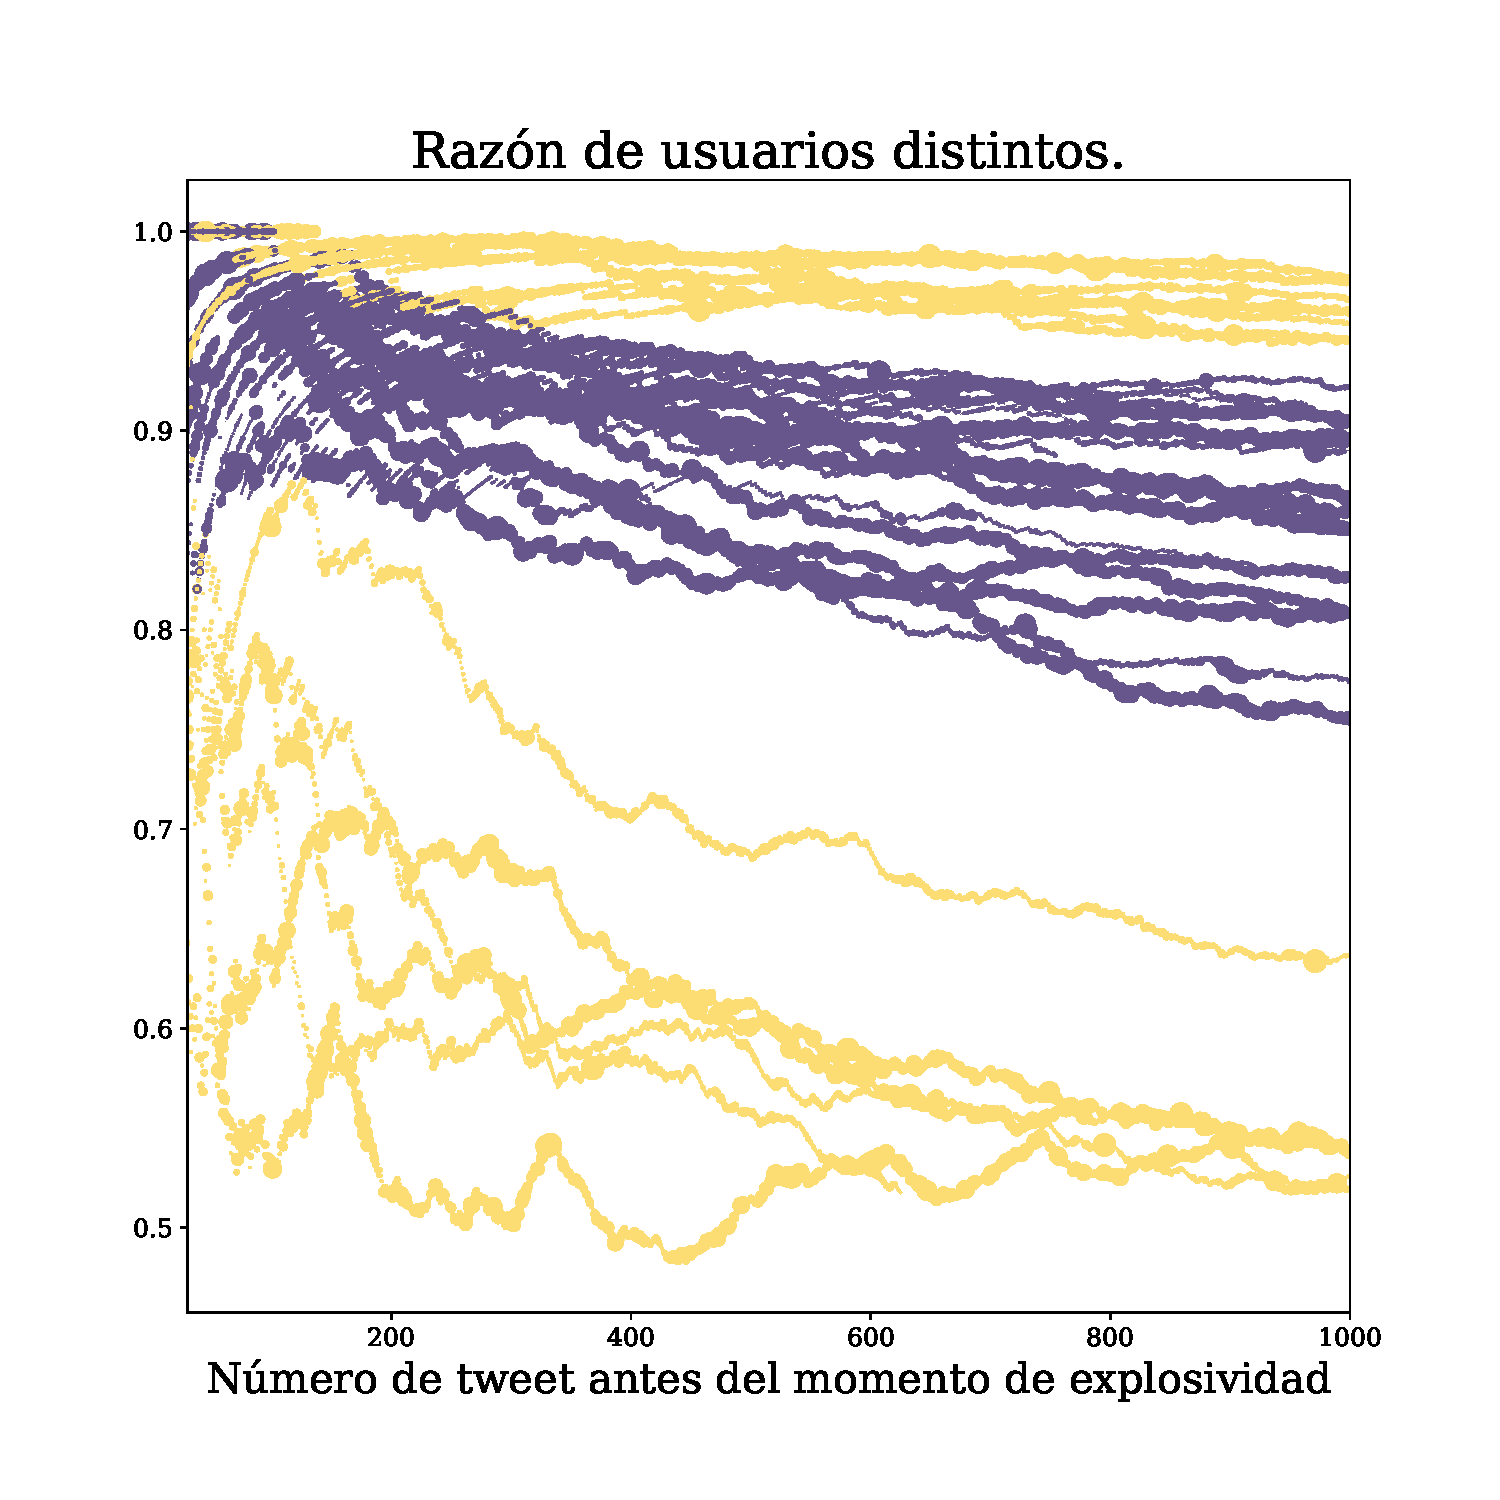
\includegraphics[scale = 0.5]{images/razonusuarios.pdf}
    \caption{ Comparativo de tendencias por los primeros 1000 tweets. Razón de usuarios nuevos en cada tweet de los 1000 tweets antes del periodo $t^{*}$. Las líneas de color morado corresponden a tendencias con comportamiento explosivo.  } 
    \label{fig:resultados_1000Tweets}
\end{figure}
 

% Sin numeroacion


\end{document}



% Esto último puede ser consecuencia del tipo de tendencia; del artículo \cite{REDDIT} nos dan un pequeño análisis de comunidades sobre \textit{subreddits} (comunidades más pequeñas) mostrando que aquellas con pocas personas pero con una organización clave entre las demás, pueden generar enfrentamientos masivos; misma idea fue hecha \cite{Conover_Ratkiewicz_Francisco_Goncalves_Menczer_Flammini_2011}, sobre discusiones políticas en \textit{Twitter}. Lo cual, al considerar la poca incertidumbre de la entropía de Shannon, es consistente con la bibliografía de comunidades pequeñas pero organizadas. 


Más aún, a sabiendas que muchas de las interacciones iniciales ocurrieron en comunidades \textit{a priori} disconexas, pero con un comportamiento comprometido \cite{D_weng2014predicting} y, justo en el momento de mayor interacción, muchas de las métricas de centralidad parecieran incremetarse y tomar mayor significancia \cite{Chng2015_bottom-up}. 